\section{Result and insight}

The result are taken from the training notebooks. Table \ref{tab:models} show the result of our training on QQP dataset. These result are evaluated on the test set, which is only a subset of the QQP dataset. The time in the table is the seconds it take to run inference of the test set.

\begin{table}[ht]
\centering
\begin{tabular}{lccccc}
    \hline
    Model & Accuracy & Precision & Recall & F1-score & Time (second) \\
    \hline
    BERT     & 0.8969 & 0.8488 & 0.8746 & 0.8561 & 276 \\
    SBERT(1) & 0.7740 & 0.6514 & 0.8333 & 0.7312 & 48  \\
    SBERT(2) & 0.8921 & 0.8331 & 0.8880 & 0.8536 & 69  \\
    \hline
\end{tabular}
\caption{Performance comparison of BERT and SBERT models}
\label{tab:models}
\end{table}

 We can see that BERT has the highest metrics on accuracy, precision, and F1-score, with SBERT(2) coming at a close second place. SBERT(1) being zero shot and not train has the worst result out of the 3. However, SBERT(1) has the fastest inference time of the three, while BERT BASE was many time slower. This comparison is not very fair for BERT either, because we use the Tiny versions of SBERT but not the tiny version of BERT, so this result is just for reference.

Our experiment were not able to meaningfully explore the aspact of finding similar semantic sentences, as the provided dataset already give us pairs of positive/negative questions, so we don't have to find the correct pair, which would emphasize the difference of $\frac{n(n-1)}{2}$ inference issue mention at the start. 

Comparing to the BERT paper's f1 score of 0.712 on QQP, we can say that we did achive better numbers, though only on a subset of the dataset.



The logic for drawing graph are in \texttt{source/graph.ipynb}. Below in figure \ref{fig:bert_01} and \ref{fig:sbert_01} are some graph taken from Tensorboard of the training process of BERT and SBERT, which can be invoke with ``\texttt{tensorboard --logdir .}''

For BERT, the graph show the training process, and for SBERT, the graph only show the training process for approach 2, because we do not train the model in approach 1.

Both training process were allowed a maximum epoch of 3, however they both early stopped during their second epochs. This suggest that the pretrained model already has strong capability to represent language without needing much fine tuning. Almost all graphs show that the metrics are very noisy during training and functuate rapidly, which suggest that it might need learning rate scheduler, which is currently missing in our training configuration. On the other hand, we might need to test fine tuning only the classifier (linear probing) in the future, which could be faster and might lead to better results.





\begin{figure}[!h]
    \centering
    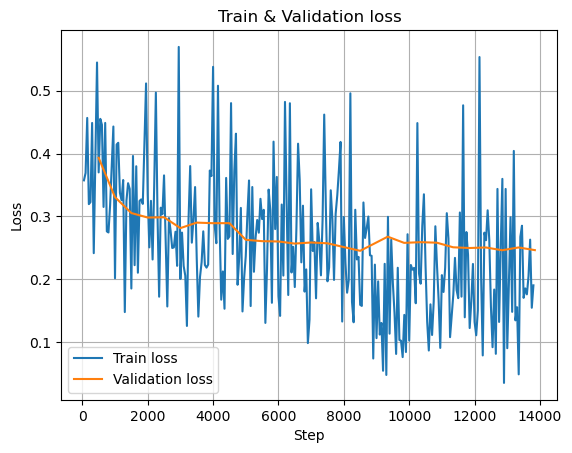
\includegraphics[width=0.49\linewidth]{image/bert_01.png}
    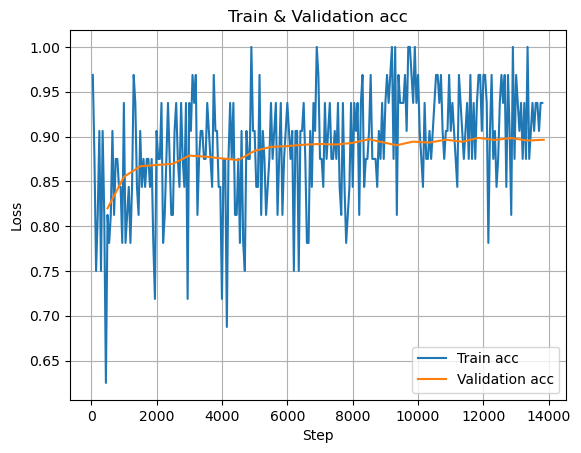
\includegraphics[width=0.49\linewidth]{image/bert_02.png}
    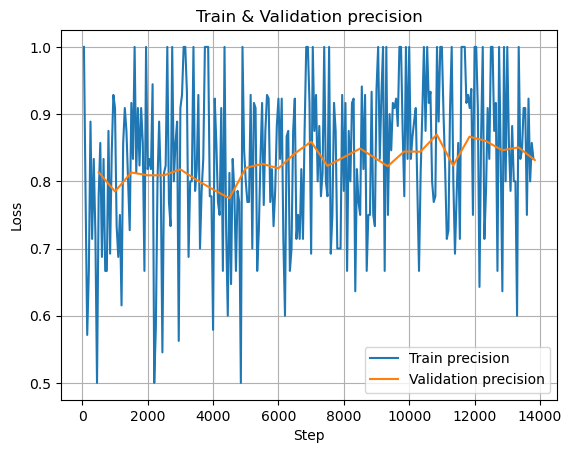
\includegraphics[width=0.49\linewidth]{image/bert_03.png}
    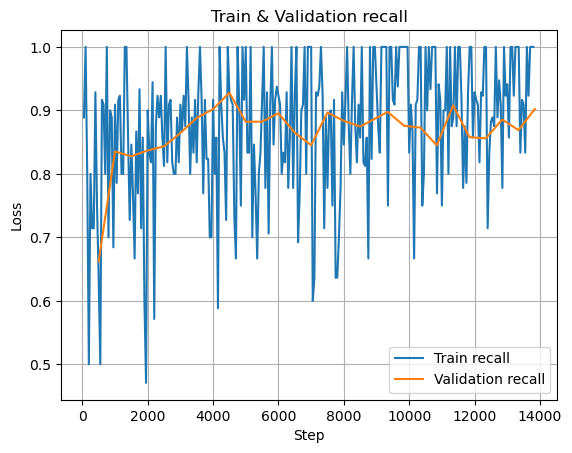
\includegraphics[width=0.49\linewidth]{image/bert_04.png}
    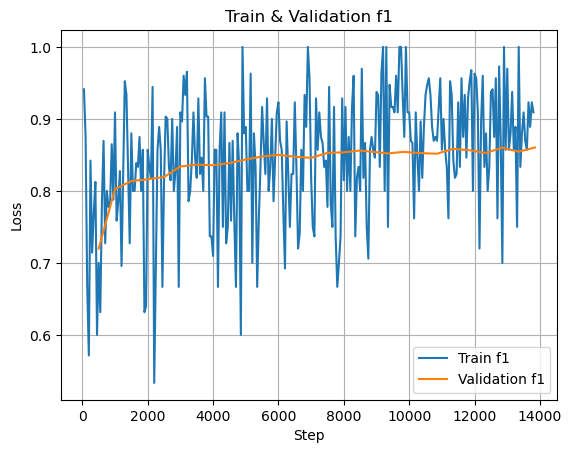
\includegraphics[width=0.49\linewidth]{image/bert_05.png}
    \caption{BERT training graph}
    \label{fig:bert_01}
\end{figure}



\begin{figure}[!h]
    \centering
    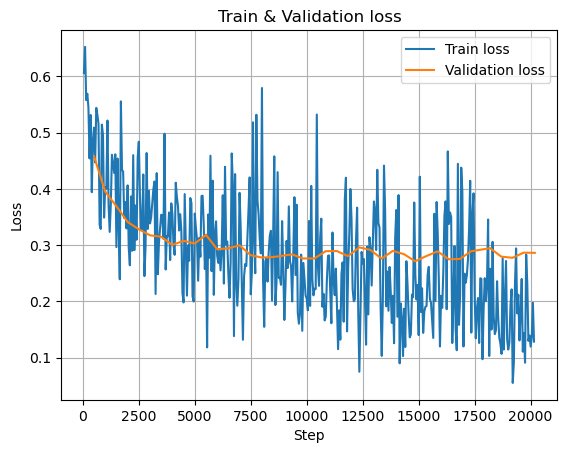
\includegraphics[width=0.49\linewidth]{image/sbert_01.png}
    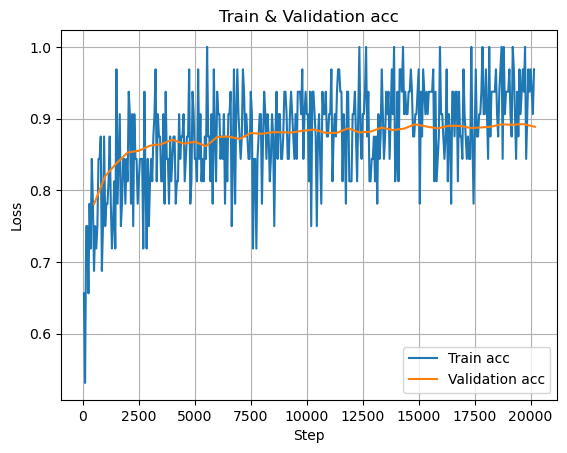
\includegraphics[width=0.49\linewidth]{image/sbert_02.png}
    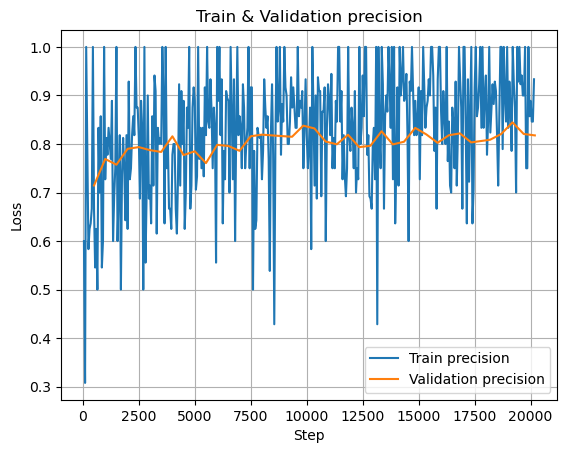
\includegraphics[width=0.49\linewidth]{image/sbert_03.png}
    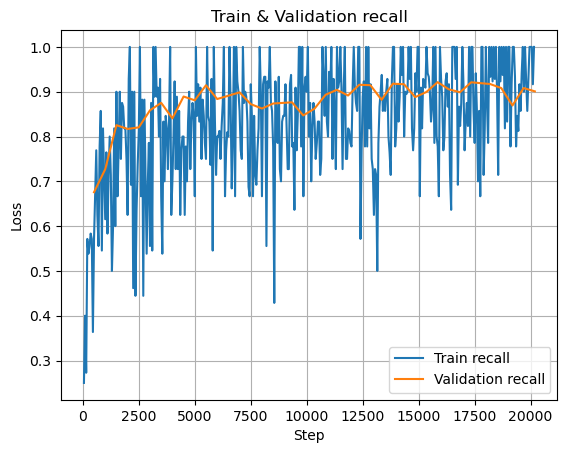
\includegraphics[width=0.49\linewidth]{image/sbert_04.png}
    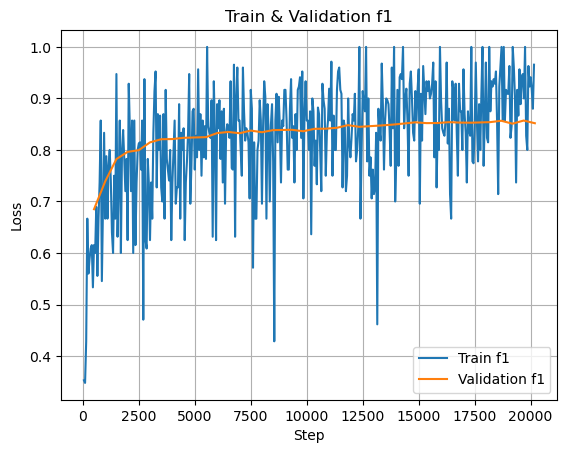
\includegraphics[width=0.49\linewidth]{image/sbert_05.png}
    \caption{SBERT training graph}
    \label{fig:sbert_01}
\end{figure}

\text{}
\newpage
\text{}
\newpage
\text{}
\newpage